% Welcome! This is the unofficial University of Udine beamer template.

% See README.md for more informations about this template.

% This style has been developed following the "Manuale di Stile"
% (Style Manual) of the University of Udine. You can find the
% manual here: https://www.uniud.it/it/ateneo-uniud/ateneo-uniud/identita-visiva/manuali-immagine-stile/manuale-stile

% Note: for some reason, the RGB values specified in the manual
% do NOT render correctly in Beamer, so they have been redefined
% for this document using the high level chromo-optic deep neural 
% quantistic technology offered by Microsoft Paint's color picker.

% We defined four theme colors: UniBrown, UniBlue, UniGold
% and UniOrange. For example, to write some uniud-brownish
% text, just use: \textcolor{UniBrown}{Hello!}

% Note that [usenames,dvipsnames] is MANDATORY due to compatibility
% issues between tikz and xcolor packages.

\documentclass[usenames,dvipsnames,xcolor=table]{beamer}
\usepackage[utf8]{inputenc}
\usepackage{tikz}
\usetikzlibrary{calc, shapes.misc}
\usepackage{verbatim}
\usetheme{uniud}

%%% Bibliography
\usepackage[style=authoryear,backend=biber]{biblatex}
\addbibresource{bibliography.bib}

% Author names in publication list are consistent 
% i.e. name1 surname1, name2 surname2
% See https://tex.stackexchange.com/questions/106914/biblatex-does-not-reverse-the-first-and-last-names-of-the-second-author
\DeclareNameAlias{author}{given-family}

%%% Suppress biblatex annoying warning
\usepackage{silence}
\WarningFilter{biblatex}{Patching footnotes failed}

%%% Some useful commands
% pdf-friendly newline in links
\newcommand{\pdfnewline}{\texorpdfstring{\newline}{ }} 
% Fill the vertical space in a slide (to put text at the bottom)
\newcommand{\framefill}{\vskip0pt plus 1filll}


\title[Steel defect detection]{An effective approach to steel defect detection}
\date[\today]{\today}
\author[Antonio Terpin e Claudio Verardo]{
  Antonio Terpin e Claudio Verardo
}
\institute{Scuola Superiore, University of Udine}

\begin{document}

\begin{frame}
\titlepage
\end{frame}

\begin{frame}{Outline}
\tableofcontents
\end{frame}

\section{Introduction}
    \begin{frame}{Introduction}
        \begin{abstract}
            Quality control is a main issue in any industry, and the automation of quality control process has become a hot topic in research. In this paper an effective solution to defect detection on steel surfaces from images is presented.
        \end{abstract}
        \vskip 0.5cm
        \begin{description}
            \item<1->[1.] Case study
            \item<2->[2.] Wavelet
            \item<3->[3.] Computer vision
        \end{description}
    \end{frame}
    % \subsection{Wavelet Analysis}
    \framepic{graphics/wavelets/wavelet}{
        \framefill
        \textcolor{black}{Wavelet}
        \vskip 0.5cm
    }

    \begin{frame}{Multi Resolution Analysis}
        \centering
        \onslide <1-> {
            \begin{block}{Goal}
                Approximate vectors of $L^2\left(\mathbb{R}\right)$ with variable degrees of resolution.
            \end{block}
        }
        \only <2> {
            \includegraphics[width=.6\textwidth]{graphics/wavelets/mra}
        }
        \only <3> {
            \includegraphics[width=.6\textwidth]{graphics/wavelets/mra-1}
        }
        \only <4> {
            \includegraphics[width=.6\textwidth]{graphics/wavelets/mra-2}
        }
        \only <5> {
            \includegraphics[width=.6\textwidth]{graphics/wavelets/mra-3}
        }
    \end{frame}

    \begin{frame}{Multi Resolution Analysis}
        \begin{block}{Axioms}
            \begin{equation}
                \cdots \subset V_{-2} \subset V_{-1} \subset V_0 \subset V_1 \subset V_2 \subset \cdots
            \end{equation}
            \begin{equation}
                \overline{\bigcup\limits_{n \in \mathbb{Z}} V_n} = L^2\left(\mathbb{R}\right)
            \end{equation}
            \begin{equation}
                \bigcap\limits_{n \in \mathbb{Z}} V_n = \left\{0\right\}
            \end{equation}
            \begin{equation}
                V_{n+1} = \mathcal{S}V_n
            \end{equation}
            \begin{equation}
                V_0 = \langle \left\{\tau^i\phi, i \in \mathbb{Z}\right\} \rangle \quad \exists \phi \in L^2\left(\mathbb{R}\right)\rangle
            \end{equation}
        \end{block}
    \end{frame}

    \begin{frame}{Multi Resolution Analysis}
        \begin{block}{Scaling function}
            \begin{equation}
                V_1 \supset V_0, \phi \in V_1
            \end{equation}
            \begin{equation}
                \left\{\mathcal{S}\tau^i\phi = \tau^{i/2}\mathcal{S}\phi, i \in \mathbb{Z}\right\} \; \text{orthonormal basis of } V_1
            \end{equation}
            \begin{equation}
                    \phi = \sum_{i \in \mathbb{Z}} g_i \tau^{i/2} \mathcal{S} \phi
            \end{equation}
        \end{block}
    \end{frame}

    \begin{frame}{Multi Resolution Analysis}
        \begin{block}{Wavelet}
            \begin{equation}
                V_{n+1} \supset V_n \Rightarrow \exists W_n \colon V_{n+1} = V_n \oplus W_n
            \end{equation}
            \begin{equation}
                \left\{\tau^i\psi\right\}_{i \in \mathbb{Z}} = W_0
            \end{equation}
            \begin{equation}
                \psi = \sum_{i \in \mathbb{Z}} h_i \tau^{i/2}\mathcal{S}\phi\quad\psi \in V_1
            \end{equation}
            \begin{equation}
                \langle \psi, \tau^i \psi \rangle = \delta_i
            \end{equation}
            \begin{equation}
                \langle \tau^j\psi, \tau^i \phi \rangle = 0
            \end{equation}
        \end{block}
    \end{frame}

    \begin{frame}
        \frametitle{Multi Resolution Analysis}
        \framesubtitle{Filter banks}
        \centering 
        \begin{tikzpicture}
            % High res
            \node[anchor= west] (highres) at (0,0) {$V_{n+1}$};
            % Low res
            \node[rectangle, draw, anchor= west, minimum height=0.75cm, minimum width=1.5cm] (g) at (3,2) {g};
            \node[circle, draw, anchor= west] (downsampleg) at (6,2) {$\downarrow 2$};
            \node[anchor= west] (lowres) at (8,2) {$V_n$};
            % Details
            \node[rectangle, draw, anchor= west, minimum height=0.75cm, minimum width=1.5cm] (h) at (3,-2) {h};
            \node[circle, draw, anchor= west] (downsampleh) at (6,-2) {$\downarrow 2$};
            \node[anchor= west] (details) at (8,-2) {$W_n$};

            \draw[->] (1,0) -- (2,0) -- (2,2) -- (3,2);
            \draw[->] (1,0) -- (2,0) -- (2,-2) -- (3,-2);

            \draw[->] (4.5,2) -- (6,2);
            \draw[->] (4.5,-2) -- (6,-2);

            \draw[->] (7,2) -- (8,2);
            \draw[->] (7,-2) -- (8,-2);

        \end{tikzpicture}
    \end{frame}

    \begin{frame}
        \frametitle{Wavelet: Example application}
        \framesubtitle{Detect abrupt changes}

        \centering
        \vskip -1cm
        $$s_1(t) = 2\sin\left(2\pi 10f_0 t\right) + \sin\left(2\pi 50f_0 t\right) + 10\delta\left(t - \frac{1}{2f_0}\right)$$
        \only<1> {
            \includegraphics[height=0.6\textheight]{graphics/wavelets/signal1}
        }
        \only<2> {
            \begin{columns}[onlytextwidth]
                \column{0.5\textwidth}
                \includegraphics[width=\textwidth]{graphics/wavelets/detect-abrupt-changes-fft}
                \column{0.5\textwidth}
                \includegraphics[width=\textwidth]{graphics/wavelets/detect-abrupt-changes-cwt}
            \end{columns}
        }

    \end{frame}

    \begin{frame}
        \frametitle{Wavelet: Example application}
        \framesubtitle{Detect temporal trends}
        $$f_{s_2} = e^t;\quad s_2 = \sin\left(2*pi*f_{s_2}t\right)$$
        \begin{columns}[onlytextwidth]
            \column{0.5\textwidth}
            \only<1-2> {
                \includegraphics[width=\textwidth]{graphics/wavelets/frequency-signal-2}
            }
            \only<3-4> {
                \includegraphics[width=\textwidth]{graphics/wavelets/detect-pattern-fft}
            }
            \column{0.5\textwidth}
            \only<2> {
                \includegraphics[width=\textwidth]{graphics/wavelets/signal2}
            }
            \only<4> {
                \includegraphics[width=\textwidth]{graphics/wavelets/detect-pattern-cwt}
            }
        \end{columns}
        
    \end{frame}


    \subsection{Computer Vision}
    \framepic{graphics/computervision/computer-vision}{
        \framefill
        \textcolor{white}{Computer Vision}
        \vskip 0.5cm
    }
    \begin{frame}{Computer Vision}
        \begin{block}{Classification Task}
            To determine to which of a set of \textbf{categories} a given object belongs to.
        \end{block}
        \begin{columns}[onlytextwidth]
            \column{0.3\textwidth}
            \centering
            \includegraphics[width=\textwidth]{graphics/computervision/classification-image.jpeg}
            \onslide <2-> {
                \column{0.4\textwidth}
                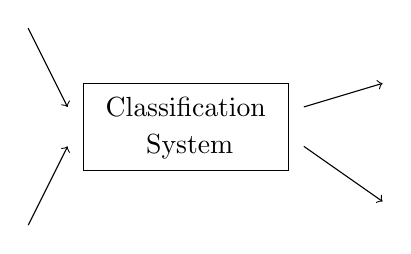
\begin{tikzpicture}
                    \node at (0,0) {Classification};
                    \node at (0.05,-0.5) {System};
                    \node[rectangle, draw, minimum width=2.6cm, minimum height=1.1cm, anchor=north west] at (-1.3,0.3) {};
                    \draw[->] (-2,1) -- (-1.5,0);
                    \draw[->] (-2,-1.5) -- (-1.5,-0.5);
                    \onslide <3-> {
                        \draw[->] (1.5,0) -- (2.5,0.3);
                        \draw[->] (1.5,-0.5) -- (2.5,-1.2);
                    }
                \end{tikzpicture}
            }
            \onslide <3-> {
                \column{0.2\textwidth}
                \vskip -0.5cm Output \vskip 0.5cm
                \begin{columns}[onlytextwidth]
                    \column{0.5\textwidth}
                        \begin{tabular}{|c|}
                            \hline
                            $0.03$\\\hline
                            \cellcolor{UniBlue}\textcolor{white}{$0.77$}\\\hline
                            $\vdots$\\\hline
                            $0.12$\\\hline
                        \end{tabular}
                    \column{0.5\textwidth}
                        \vskip -0.2cm
                        \begin{tabular}{c}
                            \\
                            \textcolor{UniBlue}{Child}\\
                            \\
                            \\
                        \end{tabular}
                \end{columns}
            }
        \end{columns}
    \end{frame}

    \begin{frame}{Computer Vision}
        \begin{block}{Object Localization Task}
            To find a given number (usually one) of items in a given context, predicting both their position and their class. \\
            \textbf{Remark.} Position is usually given as a bounding box.
        \end{block}
        \begin{columns}[onlytextwidth]
            \column{0.45\textwidth}
            \onslide <2-> {
                \includegraphics[width=\textwidth]{graphics/computervision/localization-input}
            }
            \column{0.45\textwidth}
            \onslide <3-> {
                \includegraphics[width=\textwidth]{graphics/computervision/localization-output}
            }
        \end{columns}
    \end{frame}

    \begin{frame}{Computer Vision}
        \onslide<1-> {
            \begin{block}{Object Detection Task}
                To \textbf{localize} any number of items in a given context, allowing either zero or any finite number of objects.
            \end{block}
        }
        \onslide<2-> {
            \begin{alertblock}{Remark.}
                The constraint on the number of object is \emph{a priori}. Indeed, a localization system will always look for a fixed number of objects, whereas a detection system is trained to be able to spot a variable number of objects in each input.
            \end{alertblock}
        }
    \end{frame}

    \begin{frame}{Computer Vision}
        \onslide <1-> {
            \begin{block}{Image Segmentation}
                Pixel-wide classification of the image. \textbf{Remark.} Image segmentation can be consider either the preemptive step to classification or the output of a classification system.
            \end{block}
        }
        \onslide <2-> {
            \vskip -0.5cm 
            \begin{exampleblock}{Example: Pixel-based image segmentation.}
                This family considers some distance defined over the image domain to segmentate it.
            \end{exampleblock}
        }
        \onslide <3-> {
            \vskip -0.5cm 
            \begin{exampleblock}{Example: Edge-based image segmentation.}
                This family uses an edge-detector algorithm, along with denoising and thresholding considerations, to solve the boundary detection problem.
            \end{exampleblock}
        }
    \end{frame}

    % \begin{frame}
    %     \frametitle{Pixel-based image segmentation}
    %     \framesubtitle{Whatershed}
    %     \begin{columns}[onlytextwidth]
    %         \column{0.5\textwidth}
    %         \includegraphics[width=\textwidth]{graphics/computervision/whatershed-plane}
    %         \column{0.5\textwidth}
    %         \includegraphics[width=\textwidth]{graphics/computervision/whatershed-surf}
    %     \end{columns}
    %     \only <1> {
    %         \begin{block}{Whatershed and immersion}
    %             The above pictures both show the same function defined over a 2D domain. Suppose to immerse the above right surface in some liquid, which gradually fill the two holes.
    %         \end{block}
    %     }
    %     \only <2> {
    %         \begin{block}{Whatershed and immersion}
    %             At some point the two volumes of liquid will meet, in particular they will flood at the same time over the green colored surface region.
    %         \end{block}
    %     }
    %     \only <3> {
    %         \begin{block}{Whatershed and immersion}
    %             This region is called whatershed and differentiates two areas of the image. Hence, an image can be segmentated considering its whatersheds.
    %         \end{block}
    %     }
    % \end{frame}

    % \begin{frame}
    %     \frametitle{Pixel-based image segmentation}
    %     \framesubtitle{Whatershed}
    %     % \includegraphics[width=\textwidth]{graphics/whatershed-plane}
    %     TODO insert example image\\
    %     % \includegraphics[width=\textwidth]{graphics/whatershed-surf}
    %     TODO insert example image
    % \end{frame}

    % \begin{frame}
    %     \frametitle{Pixel-based image segmentation}
    %     \framesubtitle{Whatershed}
    %     Let $\mathcal{D} \subset \mathbb{R}_+^2$ be a $2D$ domain, and $\mathcal{I} \colon \mathcal{D} \rightarrow \mathbb{R}_+$. Denote $\displaystyle h_m \triangleq \min_{\underline{x} \in \mathcal{D}}\mathcal{I}(\underline{x})$, $\displaystyle h_M \triangleq \max_{\underline{x} \in \mathcal{D}}\mathcal{I}(\underline{x})$, $T_h\left(\mathcal{I}\right) \triangleq \left\{\underline{p} \in \mathcal{D}, \mathcal{I}(\underline{p}) \leq h\right\}$.
    % \end{frame}

    % \begin{frame}
    %     \frametitle{Pixel-based image segmentation}
    %     \framesubtitle{Whatershed}
    %         \begin{itemize}
    %             \item Def, th, alg
    %             \item Example results
    %         \end{itemize}
    % \end{frame}
    \subsection{Deep Learning}
    \framepic{graphics/deeplearning/deep-learning}{
        \framefill
        \textcolor{white}{Deep Learning}
        \vskip 0.5cm
    }

    \begin{frame}{Computer Vision}
        \begin{block}{Classification Task}
            To determine to which of a set of \textbf{categories} a given object belongs to.
        \end{block}
        \begin{columns}[onlytextwidth]
            \column{0.3\textwidth}
            \centering
            \includegraphics[width=\textwidth]{graphics/computervision/classification-image.jpeg}
            \onslide <2-> {
                \column{0.4\textwidth}
                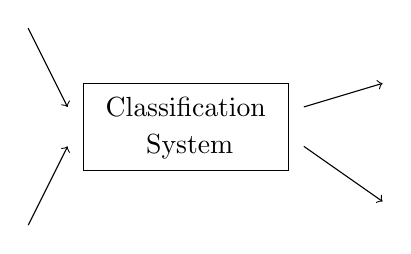
\begin{tikzpicture}
                    \node at (0,0) {Classification};
                    \node at (0.05,-0.5) {System};
                    \node[rectangle, draw, minimum width=2.6cm, minimum height=1.1cm, anchor=north west] at (-1.3,0.3) {};
                    \draw[->] (-2,1) -- (-1.5,0);
                    \draw[->] (-2,-1.5) -- (-1.5,-0.5);
                    \onslide <3-> {
                        \draw[->] (1.5,0) -- (2.5,0.3);
                        \draw[->] (1.5,-0.5) -- (2.5,-1.2);
                    }
                \end{tikzpicture}
            }
            \onslide <3-> {
                \column{0.2\textwidth}
                \vskip -0.5cm Output \vskip 0.5cm
                \begin{columns}[onlytextwidth]
                    \column{0.5\textwidth}
                        \begin{tabular}{|c|}
                            \hline
                            $0.03$\\\hline
                            \cellcolor{UniBlue}\textcolor{white}{$0.77$}\\\hline
                            $\vdots$\\\hline
                            $0.12$\\\hline
                        \end{tabular}
                    \column{0.5\textwidth}
                        \vskip -0.2cm
                        \begin{tabular}{c}
                            \\
                            \textcolor{UniBlue}{Child}\\
                            \\
                            \\
                        \end{tabular}
                \end{columns}
            }
        \end{columns}
    \end{frame}

    \begin{frame}{Computer Vision}
        \begin{block}{Object Localization Task}
            To find a given number (usually one) of items in a given context, predicting both their position and their class. \\
            \textbf{Remark.} Position is usually given as a bounding box.
        \end{block}
        \begin{columns}[onlytextwidth]
            \column{0.45\textwidth}
            \onslide <2-> {
                \includegraphics[width=\textwidth]{graphics/computervision/localization-input}
            }
            \column{0.45\textwidth}
            \onslide <3-> {
                \includegraphics[width=\textwidth]{graphics/computervision/localization-output}
            }
        \end{columns}
    \end{frame}

    \begin{frame}{Computer Vision}
        \onslide<1-> {
            \begin{block}{Object Detection Task}
                To \textbf{localize} any number of items in a given context, allowing either zero or any finite number of objects.
            \end{block}
        }
        \onslide<2-> {
            \begin{alertblock}{Remark.}
                The constraint on the number of object is \emph{a priori}. Indeed, a localization system will always look for a fixed number of objects, whereas a detection system is trained to be able to spot a variable number of objects in each input.
            \end{alertblock}
        }
    \end{frame}

    \begin{frame}{Computer Vision}
        \onslide <1-> {
            \begin{block}{Image Segmentation}
                Pixel-wide classification of the image. \textbf{Remark.} Image segmentation can be consider either the preemptive step to classification or the output of a classification system.
            \end{block}
        }
        \onslide <2-> {
            \vskip -0.5cm 
            \begin{exampleblock}{Example: Pixel-based image segmentation.}
                This family considers some distance defined over the image domain to segmentate it.
            \end{exampleblock}
        }
        \onslide <3-> {
            \vskip -0.5cm 
            \begin{exampleblock}{Example: Edge-based image segmentation.}
                This family uses an edge-detector algorithm, along with denoising and thresholding considerations, to solve the boundary detection problem.
            \end{exampleblock}
        }
    \end{frame}

    \begin{frame}{Training}
        \begin{block}{Forward propagation}
            The \emph{feedforward} neural network accepts an input $\underline{\underline{X}}$ and produce an output $\underline{y}$. The information from $\underline{\underline{X}}$ flows through the hidden units to produce $\underline{y}$. This is called \textbf{forward propagation}.
        \end{block}

        \begin{block}{Backward propagation}
            During the training the forward propagation can continue onward to evaluate a scalar cost $J\left(\underline{\underline{\theta}}\right)$. The \textbf{back-propagation} algorithm is a numerically efficient way to compute cost gradient, in order to perform gradient descent.
        \end{block}    
    \end{frame}

    \begin{frame}{Deep Learning}
        \includegraphics[width=\textwidth]{graphics/deeplearning/nn}
    \end{frame}

    \begin{frame}
        \frametitle{Training}
        \framesubtitle{Backpropagation (proof)}
        \centering
        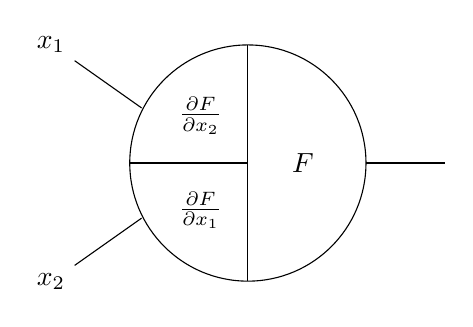
\begin{tikzpicture}
            \node[circle, draw, minimum width=3cm, minimum height=3cm] at (0,0) {};
            \node at (0.7,0) {$F$};
            \node at (-0.6,-0.6) {$\frac{\partial F}{\partial x_1}$};
            \node at (-0.6,0.6) {$\frac{\partial F}{\partial x_2}$};
            \node at (-2.5,1.5) {$x_1$};
            \node at (-2.5,-1.5) {$x_2$};

            \draw (0,0) -- (-1.5,0);
            \draw (0,-1.5) -- (0,1.5);
            \draw (1.5, 0) -- (2.5,0);

            \draw (-1.35, 0.7) -- (-2.2,1.3);
            \draw (-1.35, -0.7) -- (-2.2,-1.3);
        \end{tikzpicture}

        \vskip 0.5cm
        
        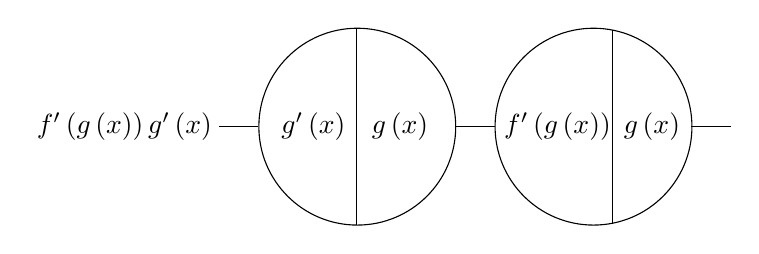
\begin{tikzpicture}
            \node at (-.7,0) {$f'\left(g\left(x\right)\right)g'\left(x\right)$};

            \draw (0.5,0) -- (1,0);

            \node[circle, draw, minimum width=2.5cm, minimum height=2.5cm, anchor=west] at (1,0) {};
            \node at (1.7, 0) {$g'\left(x\right)$};
            \node at (2.8, 0) {$g\left(x\right)$};
            \draw (2.25, 1.25) -- (2.25, -1.25);

            \draw (3.5, 0) -- (4, 0);

            \node[circle, draw, minimum width=2.5cm, minimum height=2.5cm, anchor=west] at (4,0) {};
            \node at (4.8, 0) {$f'\left(g\left(x\right)\right)$};
            \node at (6, 0) {$g\left(x\right)$};
            \draw (5.5, 1.23) -- (5.5, -1.23);

            \draw (6.5, 0) -- (7, 0);

        \end{tikzpicture}
    \end{frame}

    \begin{frame}{Convolutional Networks}
        \includegraphics[width=\textwidth]{graphics/deeplearning/cnn}
        \vskip 0.5cm
        \begin{exampleblock}{Motivation}
            \begin{enumerate}
                \item Sparse interactions
                \item Parameter sharing
                \item Equivariant representations
                \item Biologically inspired artificial intelligence
            \end{enumerate}
        \end{exampleblock}
    \end{frame}

    \begin{frame}{Convolutional Networks}
        \includegraphics[width=\textwidth]{graphics/deeplearning/cnn}
        \onslide <1-> {
            \begin{block}{Convolutional neural networks (CNN)}
                CNNs are a specialized kind of neural network for processing data that has a known grid-like topology.
            \end{block}
        }
        \onslide <2-> {
            \begin{block}{Convolutional neural networks (CNN) - 2}
                CNNs are neural networks that use convolution in place of general matrix multiplication in at least one of their layers.
            \end{block}
        }
    \end{frame}


\section{Defect detection}

\framepic{graphics/architecture/defect-detection}{
    \framefill
    \textcolor{white}{An effective approach to steel defect detection}
    \vskip 0.5cm
}

\begin{frame}{Defect detection on steel surfaces}
    \onslide <1-> {
        \includegraphics[width=\textwidth]{graphics/architecture/architecture-input}
    }
    \onslide <2-> {
        \includegraphics[width=\textwidth]{graphics/architecture/architecture-output}
    }
\end{frame}

\subsection{Data Analysis}
    \framepic{graphics/defects/dataanalysis}{
        \framefill
        \textcolor{black}{Data Analysis}
        \vskip 0.5cm
    }

    \begin{frame}
        \frametitle{Data Analysis}
        \framesubtitle{Data augmentation}
        TODO fix statistics image
    \end{frame}

    \begin{frame}
        \frametitle{Data Analysis}
        \framesubtitle{Defect analysis}
        \includegraphics[width=\textwidth]{graphics/defects/class1surface}\\
        \includegraphics[width=\textwidth]{graphics/defects/class1surface-highlighted}\\
        \includegraphics[width=\textwidth]{graphics/defects/class1shape}
    \end{frame}

    \begin{frame}
        \frametitle{Data Analysis}
        \framesubtitle{Defect analysis}
        \includegraphics[width=\textwidth]{graphics/defects/class2surface}\\
        \includegraphics[width=\textwidth]{graphics/defects/class2surface-highlighted}\\
        \includegraphics[width=\textwidth]{graphics/defects/class2shape}
    \end{frame}

    \begin{frame}
        \frametitle{Data Analysis}
        \framesubtitle{Defect analysis}
        \includegraphics[width=\textwidth]{graphics/defects/class3surface}\\
        \includegraphics[width=\textwidth]{graphics/defects/class3surface-highlighted}\\
        \includegraphics[width=\textwidth]{graphics/defects/class3shape}
    \end{frame}

    \begin{frame}
        \frametitle{Data Analysis}
        \framesubtitle{Defect analysis}
        \includegraphics[width=\textwidth]{graphics/defects/class4surface}\\
        \includegraphics[width=\textwidth]{graphics/defects/class4surface-highlighted}\\
        \includegraphics[width=\textwidth]{graphics/defects/class4shape}
    \end{frame}
\subsection{Proposed architecture}

\framepic{graphics/architecture/architecture}{
    \framefill
    \textcolor{white}{Proposed architecture}
    \vskip 0.5cm
}

\begin{frame}[fragile]{Proposed architecture}
    \vskip -0.5cm
    \begin{block}{Region-based CNN (R-CNN)}
        \begin{itemize}
            \item Region proposals
            \item Classification
        \end{itemize}
    \end{block}
    \vskip 0.25cm
    \centering
    \begin{tikzpicture}
        % Input
        \node[rectangle, draw, minimum width=2cm, minimum height=2cm, anchor=west] at (-2,0) {Image};

        % \onslide <2-> {
            \draw[->] (0.5,0) -- (1.5,0);

            % Region proposals
            \node at (2.5,1.5) {Region proposals};
            \foreach \i in {0,...,7}
                \node[rectangle, draw, minimum width=1cm, minimum height=1cm, anchor=north west, fill=white] at (2 +\i*0.2,1-\i*0.2) {};
        % }

        % \onslide <3-> {
            \draw[->] (4.5,0) -- (5.5,0);

            % Classification
            \node at (5.5,1.5) {Class};
            \draw[->, color=UniBlue] (6.2, .8) -- (5.7, 1.25);
            \draw[color=UniBlue] (6.35,-.25) ellipse (0.25cm and 1.1cm);

            \node at (8.2,2) {Encoded};
            \node at (8.3,1.5) {Pixels};
            \draw[->, color=UniOrange] (7, .95) -- (7.5, 1.55);
            \draw[color=UniOrange] (7.6,.6) ellipse (1.1cm and 0.35cm);

            \node [matrix, anchor=north west, draw] at (6,1)
            {
                % \node {Class}; & \node {EncodedPixels};\\
                \node {$1$}; & \node {``12 13 \ldots''};\\
                \node {$2$}; & \node {``6 35 \ldots''};\\
                \node {$3$}; & \node {``''};\\
                \node {$4$}; & \node {``192 78 \ldots''};\\
            };
        % }
    \end{tikzpicture}
\end{frame}

\subsubsection{Region proposals}
\begin{frame}{Region proposals}
    TODO include original image
    TODO include edged image
    TODO include alpha-shape
    TODO include bounding boxes
\end{frame}

\begin{frame}
    \frametitle{Edge-based image segmentation}
    \framesubtitle{Edge Detection}
    \includegraphics[width=\textwidth]{graphics/computervision/edge-odd}
    \includegraphics[width=\textwidth]{graphics/computervision/edge-odd-plot}
    \begin{exampleblock}{Odd transition}
        Given a function defined on a $2D$ domain, a local odd transition is likely to describe border edge.
    \end{exampleblock}
\end{frame}

\begin{frame}
    \frametitle{Edge-based image segmentation}
    \framesubtitle{Edge Detection}
    \includegraphics[width=\textwidth]{graphics/computervision/edge-even}
    \includegraphics[width=\textwidth]{graphics/computervision/edge-even-plot}
    \begin{exampleblock}{Even transition}
        Given a function defined on a $2D$ domain, a local even transition is likely to describe a line.
    \end{exampleblock}
\end{frame}
    
\begin{frame}
    \frametitle{Edge-based image segmentation}
    \framesubtitle{Phase Congruency}
    \begin{block}{Phase-congruency model}
        Given $v_1, v_2, \ldots, v_n \in \mathcal{V}$, their phase congruency is defined as:
        \begin{equation}
            \mathcal{P} = \frac{\lvert \sum_{i} v_i \rvert}{\sum_{i} \lvert v_i \rvert}
        \end{equation}
    \end{block}
    \centering
    \includegraphics[width=0.6\textwidth]{graphics/computervision/phasecongruency}
\end{frame}

\begin{frame}
	\frametitle{Edge-based image segmentation}
	\framesubtitle{Kovesi Algorithm}
	Algorithm
\end{frame}

\begin{frame}
	\frametitle{Edge-based image segmentation}
	\framesubtitle{Hysteretic Edge Follower}
	\begin{block}{Algorithm}
	  	Let $\mathcal{I}$ be the image, $\mathcal{Q} = \left\{q \in \mathcal{I} \colon \hat{\mathcal{P}}(q) > T_{high}\right\}$, $\Omega(q)$ the set of  pixels adjacent to $q$ and $\mathcal{E} = \empty$ the set of edge pixels.
		Then, the hysteretic edge follower calculates edge pixels as:
		\begin{enumerate}
			\item $q_i \in \mathcal{Q};\; \mathcal{Q} = \mathcal{Q} \setminus \{q_i\};\;\mathcal{E} = \mathcal{E} \cup \{q_i\}$
			\item $\forall q_j \in \Omega(q_i)$ if $\hat{\mathcal{P}}(q_j) > T_{low}$ then $\mathcal{E} = \mathcal{E} \cup \{q_j\}$ and repeat $(2)$ with $q_i = q_j$
			\item if $\mathcal{Q} \neq \emptyset$ then repeat $(1)$
		\end{enumerate}
	\end{block}
\end{frame}

\begin{frame}
	\frametitle{Edge-based image segmentation}
	\framesubtitle{Hysteretic Edge Follower}
	\only<1-4> {
		\includegraphics[width=\textwidth]{graphics/architecture/detector-ex}
	}
	\only<2-4> {
		\includegraphics[width=\textwidth]{graphics/architecture/detector-ex-hysteresis-30-50}
	}
	\only<3-4> {
		\includegraphics[width=\textwidth]{graphics/architecture/detector-ex-hysteresis-60-100}
	}
	\only<4-4> {
		\includegraphics[width=\textwidth]{graphics/architecture/detector-ex-hysteresis-90-150}
	}
\end{frame}

\begin{frame}
    \frametitle{Edge-based image segmentation}
    \framesubtitle{$\alpha$-Shape}
    \begin{columns}[onlytextwidth]
        \column{0.5\textwidth}
            \onslide <1-> {
                \includegraphics[width=\textwidth]{graphics/computervision/detector-points}
            }
        \column{0.5\textwidth}
            \onslide <2-> {
                \includegraphics[width=\textwidth]{graphics/computervision/detector-a-shape-better-radius}
            }
    \end{columns}
%    \onslide <3-> {
%        \begin{theorem}[Topologically correct image segmentation]
%            Under certain conditions on the parameters of the alpha-shape, the boundary reconstruction is topologically equivalent to the boundary of the original region.
%        \end{theorem}
%    }
\end{frame}

\begin{frame}
	\frametitle{Edge-based image segmentation}
	\framesubtitle{$\alpha$-Shape}
	\only<1-3> {
			\includegraphics[width=\textwidth]{graphics/architecture/detector-ex}
	}
	\only<2-3> {
			\includegraphics[width=\textwidth]{graphics/architecture/detector-ex-segmentated}
	}
	\only<3-3> {
			\includegraphics[width=\textwidth]{graphics/architecture/detector-ex-bounding-box}
	}
\end{frame}

\begin{frame}
    \frametitle{Region proposals}
    \framesubtitle{Optimization}
    \onslide <1-> {
        \begin{alertblock}{Kovesi algorithm tuning}
            Parameters: $N$, $U$, $\lambda$ and $s$.
        \end{alertblock}
    }
    \onslide <2-> {
        \begin{alertblock}{Hysteretic edge follower tuning}
        	Parameters: $T_{low}$ and $T_{high}$.
        \end{alertblock}
    }
    \onslide <3-> {
        \begin{alertblock}{Alpha shape tuning}
        	Parameters: $\alpha$, $T_{hole}$ and $T_{regions}$.
        \end{alertblock}
    }
    \onslide <3-> {
        \begin{exampleblock}{Parameters tuning - solution}
            An empirical approach is proposed: \textbf{Bayesian optimization} is used to tune the hyper parameters of the algorithm.
        \end{exampleblock}
    }
\end{frame}

\begin{frame}
	\frametitle{Region proposals}
	\framesubtitle{Optimization}
	\begin{block}{Loss function}
		\begin{equation*}
		\mathcal{L} = 1 - 2 \frac{\lvert X \cap Y \rvert}{\lvert X \rvert + \lvert Y \rvert}
		\end{equation*}
	\end{block}
	\begin{block}{Accuracy}
		\begin{equation*}
		\mathcal{A} = \frac{\lvert X \cap Y \rvert}{\lvert Y \rvert}
		\end{equation*}
	\end{block}
\end{frame}

\begin{frame}
    \frametitle{Region proposals}
    \framesubtitle{Results}
    \vskip -0.5cm
	\begin{table}
		\centering
		\small	
		\begin{tabular}{|c|c|c|c|c|c|}
			\hline		
			\textbf{No.} & \textbf{Equal.} & \textbf{MinMax} & \textbf{Batch} & \textbf{Loss} & \textbf{Accuracy}\\ \hline
			\multirow{3}{*}{1} & no & no & 1024 & 0.8773 & 0.6234 \\
			& no & yes & 1024 & \textbf{0.8378} & \textbf{0.5477} \\
			& yes & no & 1024 & 0.9205 & 0.6752 \\
			& yes & yes & 1024 & 0.7977 & 0.4925 \\ \hline
			\multirow{3}{*}{2} & no & no & 760 & 0.9103 & 0.7318\\
			& no & yes & 760 & \textbf{0.9061} & \textbf{0.7738} \\
			& yes & no & 760 & 0.9676 & 0.9587 \\
			& yes & yes & 760 & 0.9172 & 0.3333 \\ \hline
			\multirow{3}{*}{3} & no & no & 1024 & 0.7382 & 0.6710 \\
			& no & yes & 1024 & \textbf{0.6852} & \textbf{0.6168} \\
			& yes & no & 1024 & 0.8161 & 0.9145 \\
			& yes & yes & 1024 & 0.6995 & 0.4600 \\ \hline
			\multirow{3}{*}{4} & no & no & 1024 & 0.6261 & 0.6190 \\
			& no & yes & 1024 & \textbf{0.6455} & \textbf{0.7528} \\
			& yes & no & 1024 & 0.6694 & 0.7334 \\
			& yes & yes & 1024 & 0.6050 & 0.5550 \\ \hline
		\end{tabular}
	\end{table}
\end{frame}

\begin{frame}
	\frametitle{Region proposals}
	\framesubtitle{Example: Class No.1}
    \only<1-4> {
		\includegraphics[width=\textwidth]{graphics/results/detector-result-class1-1}
	}
	\only<2-4> {
		\includegraphics[width=\textwidth]{graphics/results/detector-result-class1-2}
	}
	\only<3-4> {
		\includegraphics[width=\textwidth]{graphics/results/detector-result-class1-3}
	}
	\only<4> {
		\includegraphics[width=\textwidth]{graphics/results/detector-result-class1-4}
	}
\end{frame}

\begin{frame}
\frametitle{Region proposals}
\framesubtitle{Example: Class No.2}
	\only<1-4> {
		\includegraphics[width=\textwidth]{graphics/results/detector-result-class2-1}
	}
	\only<2-4> {
		\includegraphics[width=\textwidth]{graphics/results/detector-result-class2-2}
	}
	\only<3-4> {
		\includegraphics[width=\textwidth]{graphics/results/detector-result-class2-3}
	}
	\only<4> {
		\includegraphics[width=\textwidth]{graphics/results/detector-result-class2-4}
	}
\end{frame}

\begin{frame}
\frametitle{Region proposals}
\framesubtitle{Example: Class No.3}
	\only<1-4> {
		\includegraphics[width=\textwidth]{graphics/results/detector-result-class3-1}
	}
	\only<2-4> {
		\includegraphics[width=\textwidth]{graphics/results/detector-result-class3-2}
	}
	\only<3-4> {
		\includegraphics[width=\textwidth]{graphics/results/detector-result-class3-3}
	}
	\only<4> {
		\includegraphics[width=\textwidth]{graphics/results/detector-result-class3-4}
	}
\end{frame}

\begin{frame}
\frametitle{Region proposals}
\framesubtitle{Example: Class No.4}
	\only<1-4> {
		\includegraphics[width=\textwidth]{graphics/results/detector-result-class4-1}
	}
	\only<2-4> {
		\includegraphics[width=\textwidth]{graphics/results/detector-result-class4-2}
	}
	\only<3-4> {
		\includegraphics[width=\textwidth]{graphics/results/detector-result-class4-3}
	}
	\only<4> {
		\includegraphics[width=\textwidth]{graphics/results/detector-result-class4-4}
	}
\end{frame}

\subsubsection{MC-CNN}
\begin{frame}{Multi Column CNN (MC-CNN)}
    \centering
    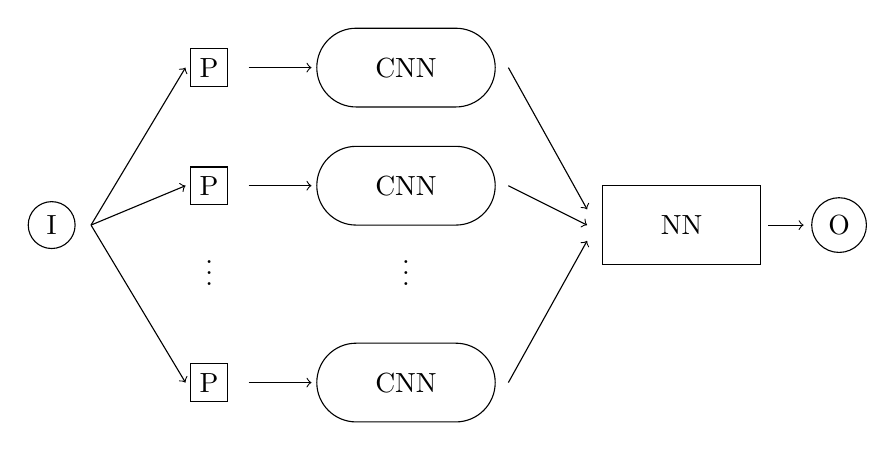
\begin{tikzpicture}
        % image
        \node[circle, draw] (input) at (0,0) {I};

        % preprocessed image
        \node[rectangle, draw] (p1) at ($(input) + (2,2)$) {P};
        \node[rectangle, draw] (p2) at ($(input) + (2,.5)$) {P};
        \node (p3) at ($(input) + (2,-.5)$) {\vdots};
        \node[rectangle, draw] (p4) at ($(input) + (2,-2)$) {P};

        % image to preprocessed image
        \draw[->] ($(input) + (0.5, 0)$) -- ($(p1) + (-0.3, 0)$);
        \draw[->] ($(input) + (0.5, 0)$) -- ($(p2) + (-0.3, 0)$);
        \draw[->] ($(input) + (0.5, 0)$) -- ($(p4) + (-0.3, 0)$);

        % cnn
        \node[rounded rectangle, draw, minimum width=2.5cm, minimum height=1cm] (cnn1) at ($(p1) + (2.5,0)$) {CNN};
        \node[rounded rectangle, draw, minimum width=2.5cm, minimum height=1cm] (cnn2) at ($(p2) + (2.5,0)$) {CNN};
        \node[minimum width=2.5cm, minimum height=1cm] (cnn3) at ($(p3) + (2.5,0)$) {\vdots};
        \node[rounded rectangle, draw, minimum width=2.5cm, minimum height=1cm] (cnn4) at ($(p4) + (2.5,0)$) {CNN};

        % preprocessed to cnn
        \draw[->] ($(p1) + (0.5, 0)$) -- ($(cnn1) + (-1.2, 0)$);
        \draw[->] ($(p2) + (0.5, 0)$) -- ($(cnn2) + (-1.2, 0)$);
        \draw[->] ($(p4) + (0.5, 0)$) -- ($(cnn4) + (-1.2, 0)$);

        % classifier
        \node[rectangle, draw, minimum width=2cm, minimum height=1cm] (classifier) at ($(cnn3) + (3.5,0.5)$) {NN};

        % cnn to classifier
        \draw[->] ($(cnn1) + (1.3, 0)$) -- ($(classifier) + (-1.2, .2)$);
        \draw[->] ($(cnn2) + (1.3, 0)$) -- ($(classifier) + (-1.2, 0)$);
        \draw[->] ($(cnn4) + (1.3, 0)$) -- ($(classifier) + (-1.2, -.2)$);

        % output
        \node[circle, draw] (output) at ($(classifier) + (2,0)$) {O};

        % classifier to output
        \draw[->] ($(classifier) + (1.1, 0)$) -- ($(output) + (-.45, 0)$);

    \end{tikzpicture}
\end{frame}

\begin{frame}{Multi Column CNN (MC-CNN)}
    \includegraphics[width=\textwidth]{graphics/architecture/mc-cnn-input}
    $$\Downarrow$$
    \centering
    \begin{tabular}{|c|c|c|c|c|}
        \hline
        Flawless area & Defect \#1 & Defect \#2 & Defect \#3 & Defect \#4\\\hline
        $1\%$ & $4\%$ & $6\%$ & \cellcolor{UniBlue}\textcolor{white}{$87\%$} & $2\%$ \\
        \hline
    \end{tabular}
\end{frame}

% \begin{frame}
%     \frametitle{Multi Column CNN (MC-CNN)}
%     \framesubtitle{Shape column}
%     \includegraphics[width=\textwidth]{graphics/architecture/mc-cnn-shape}
%     % \includegraphics[width=\textwidth]{graphics/architecture/mc-cnn-shape-architecture}
%     TODO confusion matrix + learning curve
% \end{frame}

% \begin{frame}
%     \frametitle{Multi Column CNN (MC-CNN)}
%     \framesubtitle{Local column}
%     \includegraphics[width=\textwidth]{graphics/architecture/mc-cnn-local}
%     % \includegraphics[width=\textwidth]{graphics/architecture/mc-cnn-shape-architecture}
%     TODO confusion matrix + learning curve
% \end{frame}

% \begin{frame}
%     \frametitle{Multi Column CNN (MC-CNN)}
%     \framesubtitle{Global column}
%     \includegraphics[width=\textwidth]{graphics/architecture/mc-cnn-global}
%     % \includegraphics[width=\textwidth]{graphics/architecture/mc-cnn-shape-architecture}
%     TODO confusion matrix + learning curve
% \end{frame}

\subsubsection{Output layer}
\begin{frame}{Output layer}
    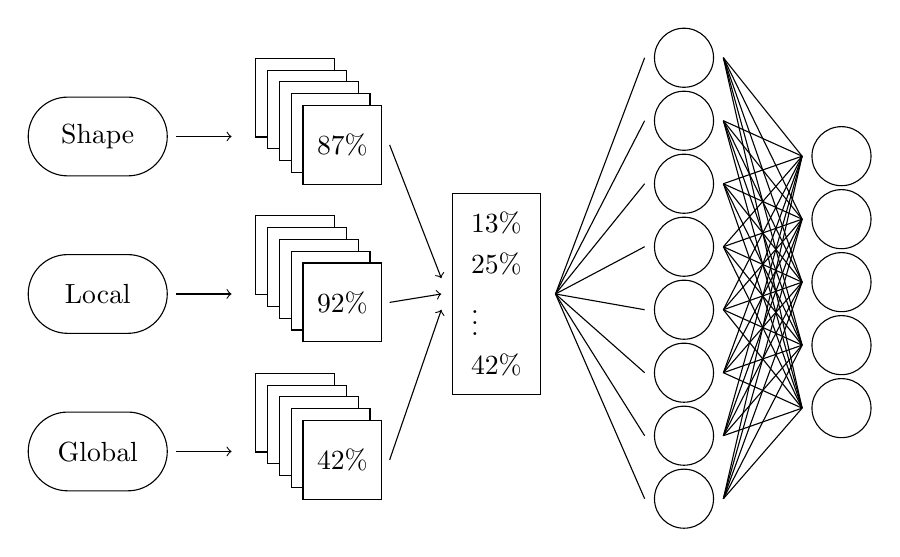
\begin{tikzpicture}

        % columns
        \node[rounded rectangle, draw, minimum width = 2cm, minimum height=1cm] (cnn1) at (0,2) {Shape};
        \node[rounded rectangle, draw, minimum width = 2cm, minimum height=1cm] (cnn2) at (0,0) {Local};
        \node[rounded rectangle, draw, minimum width = 2cm, minimum height=1cm] (cnn3) at (0,-2) {Global};

        % columns output
        \foreach \i in {0,...,4}
            \node[rectangle, draw, minimum width=1cm, minimum height=1cm, anchor=north west, fill=white] (output1 \i) at ($(cnn1) + (2+\i*0.15, 1-\i*.15) $) {$87\%$};

        \foreach \i in {0,...,4}
            \node[rectangle, draw, minimum width=1cm, minimum height=1cm, anchor=north west, fill=white] (output2 \i) at ($(cnn2) + (2+\i*0.15, 1-\i*.15) $) {$92\%$};

        \foreach \i in {0,...,4}
            \node[rectangle, draw, minimum width=1cm, minimum height=1cm, anchor=north west, fill=white] (output3 \i) at ($(cnn3) + (2+\i*0.15, 1-\i*.15) $) {$42\%$};

        % columns to output
        \draw[->] ($(cnn1) + (1, 0)$) -- ($(cnn1) + (1.7, 0)$);
        \draw[->] ($(cnn2) + (1, 0)$) -- ($(cnn2) + (1.7, 0)$);
        \draw[->] ($(cnn3) + (1, 0)$) -- ($(cnn3) + (1.7, 0)$);

        % fuse output
        \node [matrix, anchor=west, draw] (finalinput) at ($(cnn2) + (4.5,0)$)
        {
            \node {$13\%$};\\
            \node {$25\%$};\\
            \node {\vdots};\\
            \node {$42\%$};\\
        };

        % cnn output to flatten
        \draw[->] ($(output1 4) + (.6, 0)$) -- ($(finalinput) + (-.7,.2)$);
        \draw[->] ($(output2 4) + (.6, 0)$) -- ($(finalinput) + (-.7,0)$);
        \draw[->] ($(output3 4) + (.6, 0)$) -- ($(finalinput) + (-.7,-.2)$);

        % hidden layer
        \foreach \i in {0,...,7}
            \node[circle, draw, minimum width=.75cm, minimum height=.75cm, anchor=west] (h \i) at ($(finalinput) + (2, 3-\i*.8) $) {};
        \foreach \i in {0,...,7}
            \draw ($(finalinput) + (.75,0)$) -- ($(h \i) + (-.5,0)$);

        % output layer
        \foreach \i in {0,...,4}
            \node[circle, draw, minimum width=.75cm, minimum height=.75cm, anchor=west] (o \i) at ($(finalinput) + (4, 1.75-\i*.8) $) {};
        \foreach \i in {0,...,4}
            \foreach \j in {0,...,7}
                \draw ($(h \j) + (.5,0)$) -- ($(o \i) + (-.5,0)$);
        
        
    \end{tikzpicture}
    % FC NN + bayesopt params....
\end{frame}

\begin{frame}
    \frametitle{Multi Column CNN (MC-CNN)}
    \framesubtitle{Local column}
    \begin{columns}
        \column{.5\textwidth}
            Hello
%        \only<2> {
%            \column{.25}
%                % \includegraphics[height=\linewidth, angle=90, origin=c]{graphics/architecture/act_net}
%            \column{.25}
%                % \includegraphics[height=\linewidth, angle=90, origin=c]{graphics/architecture/act_net_hope}
%        }
    \end{columns}
\end{frame}


\subsection{Challenger}
\begin{frame}
    \frametitle{Challenger}
    \framesubtitle{Sliding window}
    \centering
    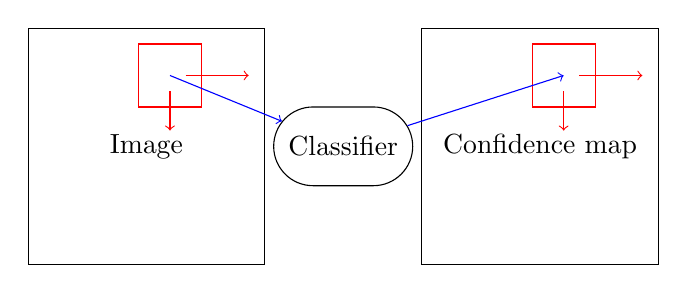
\begin{tikzpicture}
        % Image
        \node[rectangle, draw, minimum width=3cm, minimum height=3cm] (image) at (0,0) {Image};
        % Window
        \node[rectangle, draw=red, minimum width=.8cm, minimum height=.8cm] (window) at ($(image) + (.3,.9)$) {};
        % Sliding window
        \draw[->, draw=red] ($(window) + (.2,0)$) -- ($(window) + (1,0)$);
        \draw[->, draw=red] ($(window) + (0,-.2)$) -- ($(window) + (0,-.7)$);
        % Classifier
        \node[rounded rectangle, draw, minimum width=2cm, minimum height=1cm] (classifier) at ($(image) + (2.5,0)$) {Classifier};
        \draw[->,draw=blue] ($(window) + (0,0)$) -- (classifier);
        % Confidence map
        \node[rectangle,draw,minimum width=3cm, minimum height=3cm] (confidence map) at ($(classifier) + (2.5,0)$) {Confidence map};
        \node[rectangle, draw=red, minimum width=.8cm, minimum height=.8cm] (confidence map window) at ($(confidence map) + (.3,.9)$) {};
        \draw[->, draw=red] ($(confidence map window) + (.2,0)$) -- ($(confidence map window) + (1,0)$);
        \draw[->, draw=red] ($(confidence map window) + (0,-.2)$) -- ($(confidence map window) + (0,-.7)$);
        \draw[->,draw=blue] (classifier) -- ($(confidence map window)$);
    \end{tikzpicture}
\end{frame}

% \begin{frame}
%     \frametitle{Challenger}
%     \framesubtitle{Landmarks}
% \end{frame}
\section{Results}
    \begin{frame}
        \frametitle{Results}
        \framesubtitle{Local Column}
        \centering
        \begin{columns}
            \column{0.5\textwidth}
                \onslide <1-> {
                    \includegraphics[width=\linewidth]{graphics/results/spreader-net-confusion-noneq}
                }
            \column{0.5\textwidth}
                \onslide <2-> {
                    \includegraphics[width=\linewidth]{graphics/results/spreader-net-confusion}
                }
        \end{columns}
    \end{frame}

    \begin{frame}
        \frametitle{Results}
        \framesubtitle{Local Column}
        \centering
        \begin{columns}
            \column{0.5\textwidth}
                \onslide <1-> {
                    \includegraphics[width=\linewidth]{graphics/results/spreader-net-confusion}
                }
            \column{0.5\textwidth}
                \onslide <2-> {
                    \includegraphics[width=\linewidth]{graphics/results/crop-net-confusion}
                }
        \end{columns}
    \end{frame}

    \begin{frame}{Further work}
        \centering
        \begin{description}
            \item <1->[1.] Local-equalization
            \item <2->[2.] Deeper architectures 
            \item <3->[3.] Shape-Column, Global-Column, Final classifier
            \item <4->[4.] Challenger architecture
        \end{description}
        \vskip 1.5cm
        \onslide<3-> {
            The project can be found in the \href{https://github.com/antonioterpin/wavelet_ml}{\texttt{GitHub repository}}
            \vskip 0.5cm
            \url{https://github.com/antonioterpin/wavelet_ml}
        }
    \end{frame}

% \begin{frame}[t,allowframebreaks]
% \frametitle{Bibliography}

% \nocite{*} % will display the non-cited publications as well. Useful for a publication list.

% \printbibliography

% \end{frame}

\end{document}